\documentclass[12pt,a4paper,oneside]{article}
\usepackage[colorlinks=true, unicode]{hyperref}
\usepackage[utf8]{inputenc}
\usepackage[czech]{babel}
\usepackage{graphicx}
\usepackage{pdfpages}
\textwidth 16cm \textheight 25cm
\topmargin -1.3cm 
\oddsidemargin 0cm
\usepackage{footnote}
\pagestyle{empty}
\begin{document}
\title{Paměťový modul SDcard01B}
\author{Jakub Kákona, kaklik@mlab.cz}
\maketitle

\thispagestyle{empty}
\begin{abstract}
Modul poskytuje fyzické rozhraní pro připojení SDkaret k mikroprocesorům, nebo jiným digitálním systémům.
\end{abstract}

\begin{figure} [htbp]
\begin{center}
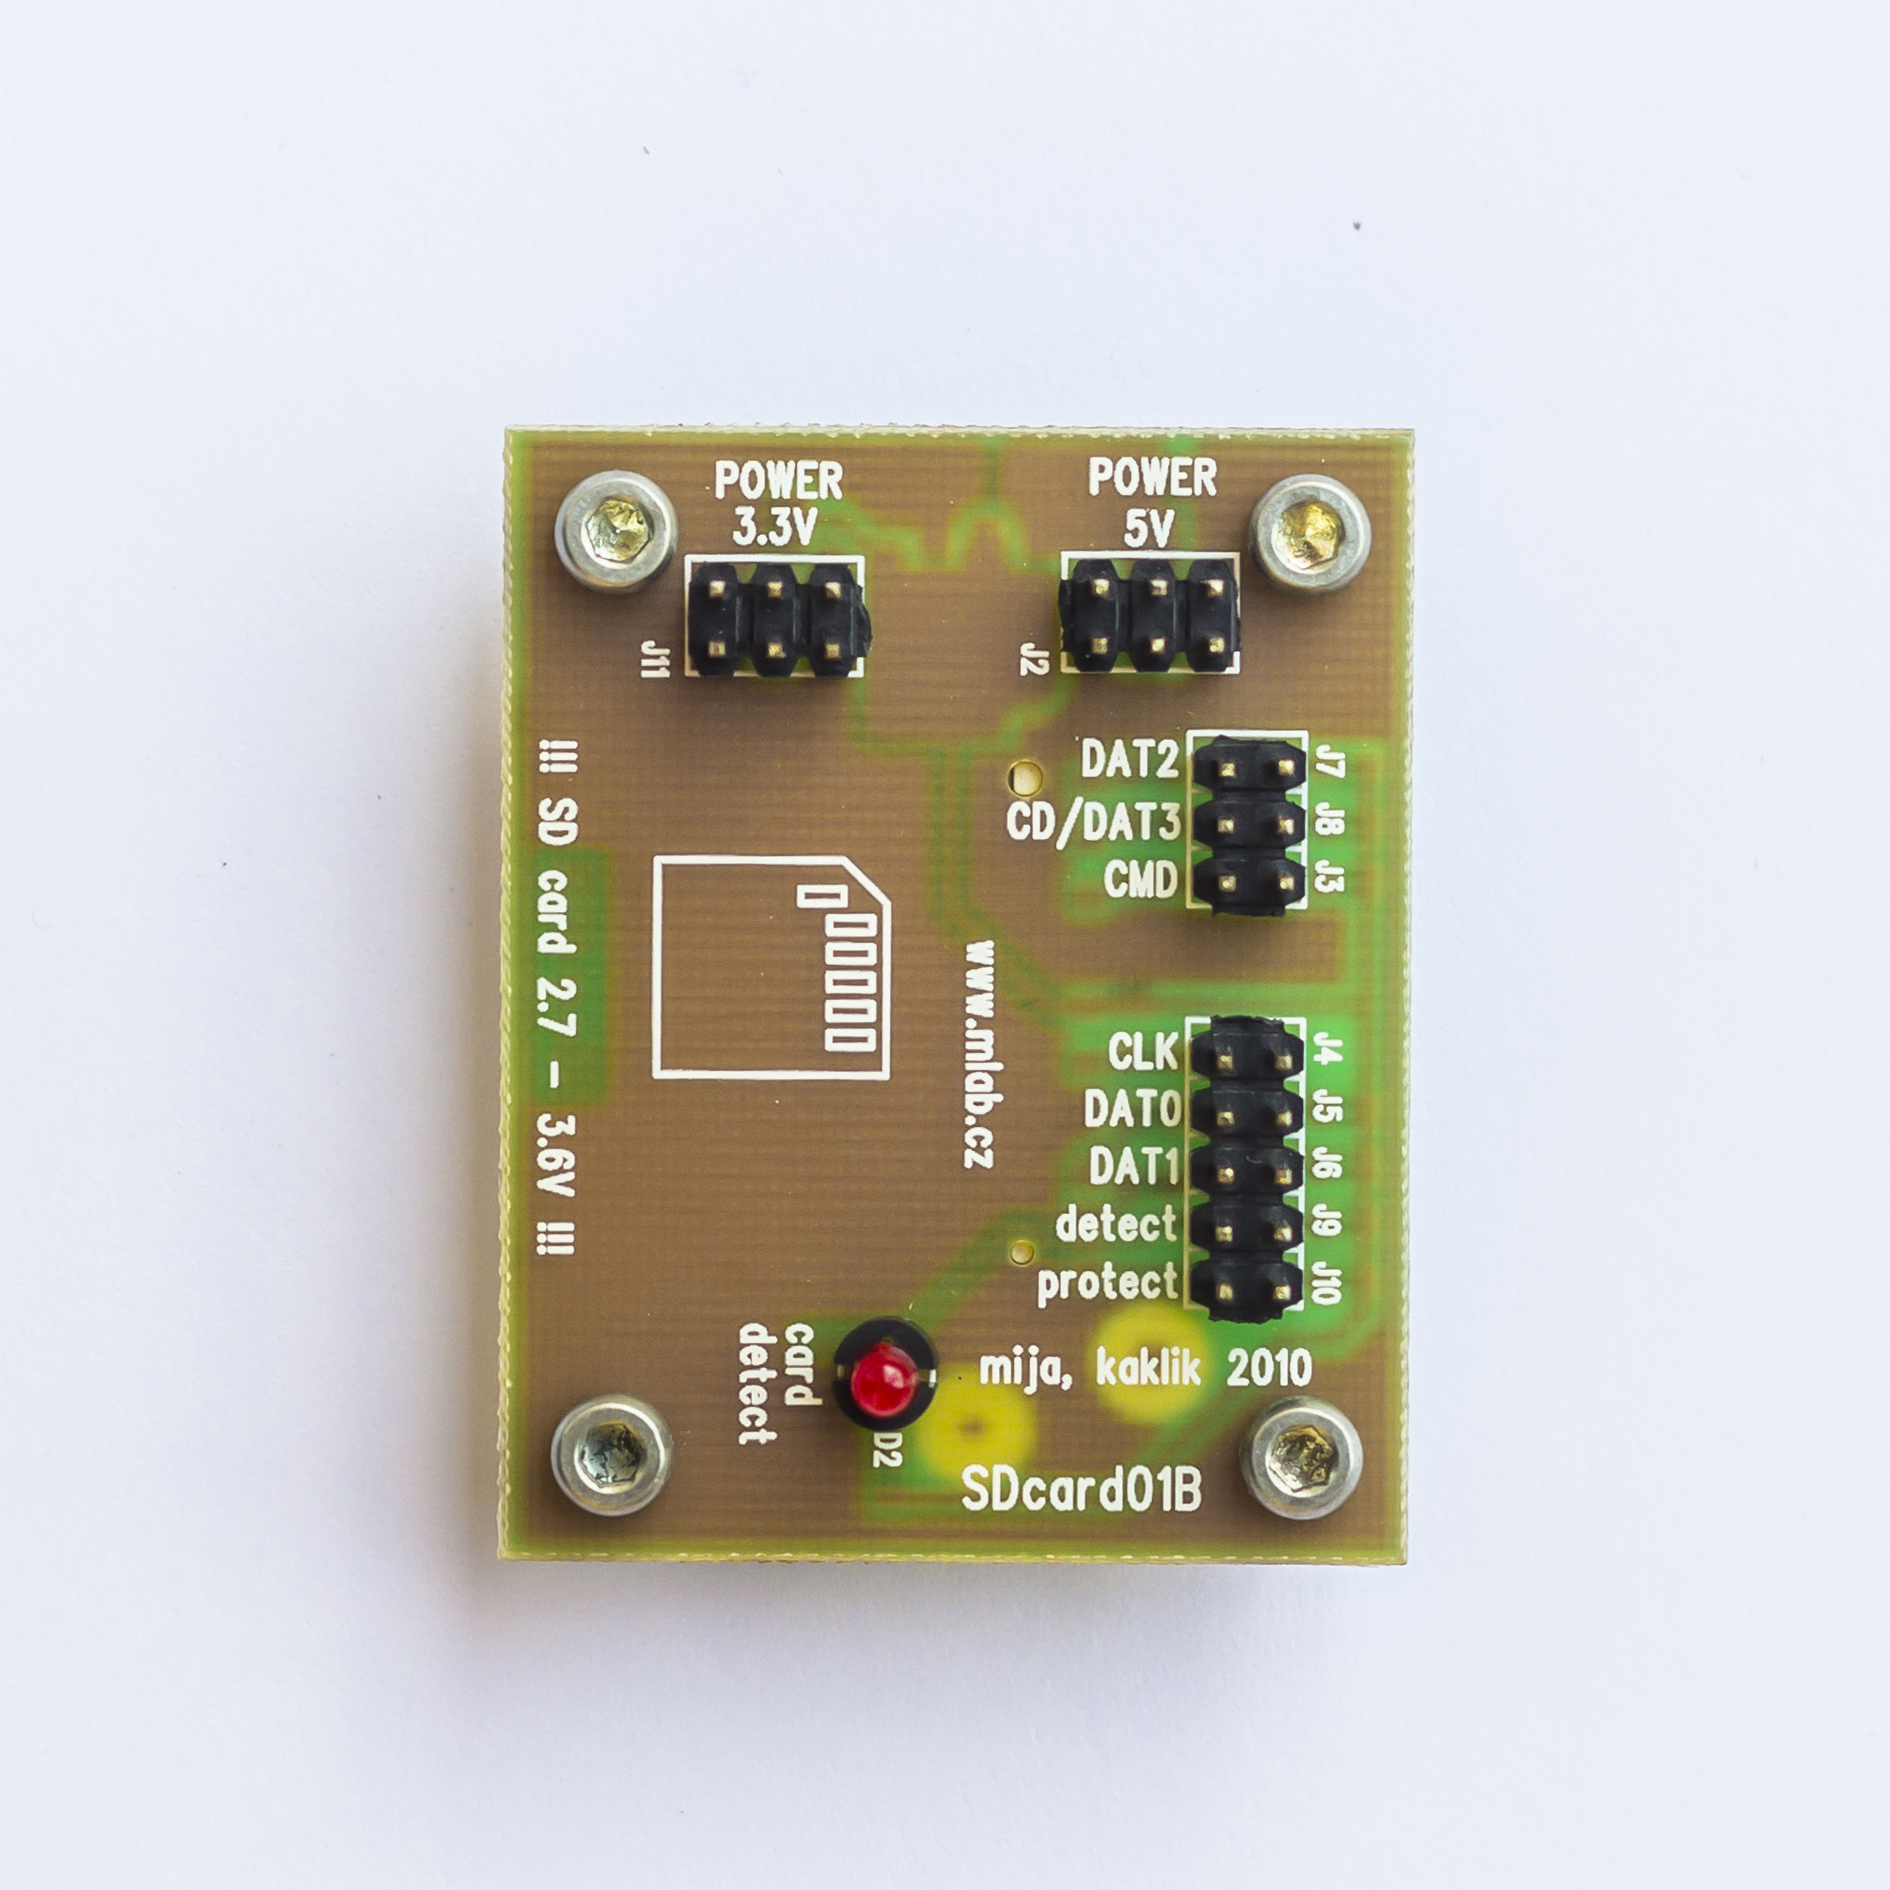
\includegraphics [width=100mm] {./img/SDCARD01B_Top_Big.jpg} 
\end{center}
\end{figure}

\begin{figure} [b]

\includegraphics [width=25mm] {./img/SDcard01B_QRcode.png} 
\end{figure}

\newpage
\tableofcontents

\section{Technické parametry}
\begin{table}[htbp]
\begin{center}
\begin{tabular}{|c|c|p{4.7cm}|}
\hline
Parametr & Hodnota & Poznámka \\
\hline
Napájecí napětí POWER  & max 5V &  Interní napájení je stabilizováno lineárním stablizátorem.\\ 
\hline
Napájecí napětí Vcore & +1,8V, 2,7V, 3,3V &  Záleží na konkrétním typu SDkarty \\ 
\hline
Digitální úrovně & CMOS &  Odpovídají logickým úrovním SDkarty \\ 
\hline
\end{tabular}
\end{center}
\end{table}

\section{Popis konstrukce}

\subsection{Zapojení}
Zapojení modulu je řešeno tak, aby umožnilo připojení řídícího mikroprocesoru provozovaného na podobném napětí jako je připojená SD-karta. Konstrukčně je tato záležitost řešena pull-up rezistory a ochrannými rezistory zařazenými sériově mezi IO piny a SDkartu. Je to řešení, které je schopno tolerovat rozdíl provozních napětí řádově v desetinách voltu. Rozhodně není určeno pro vzájemné přizpůsobení například 5V a 3V3 logiky.

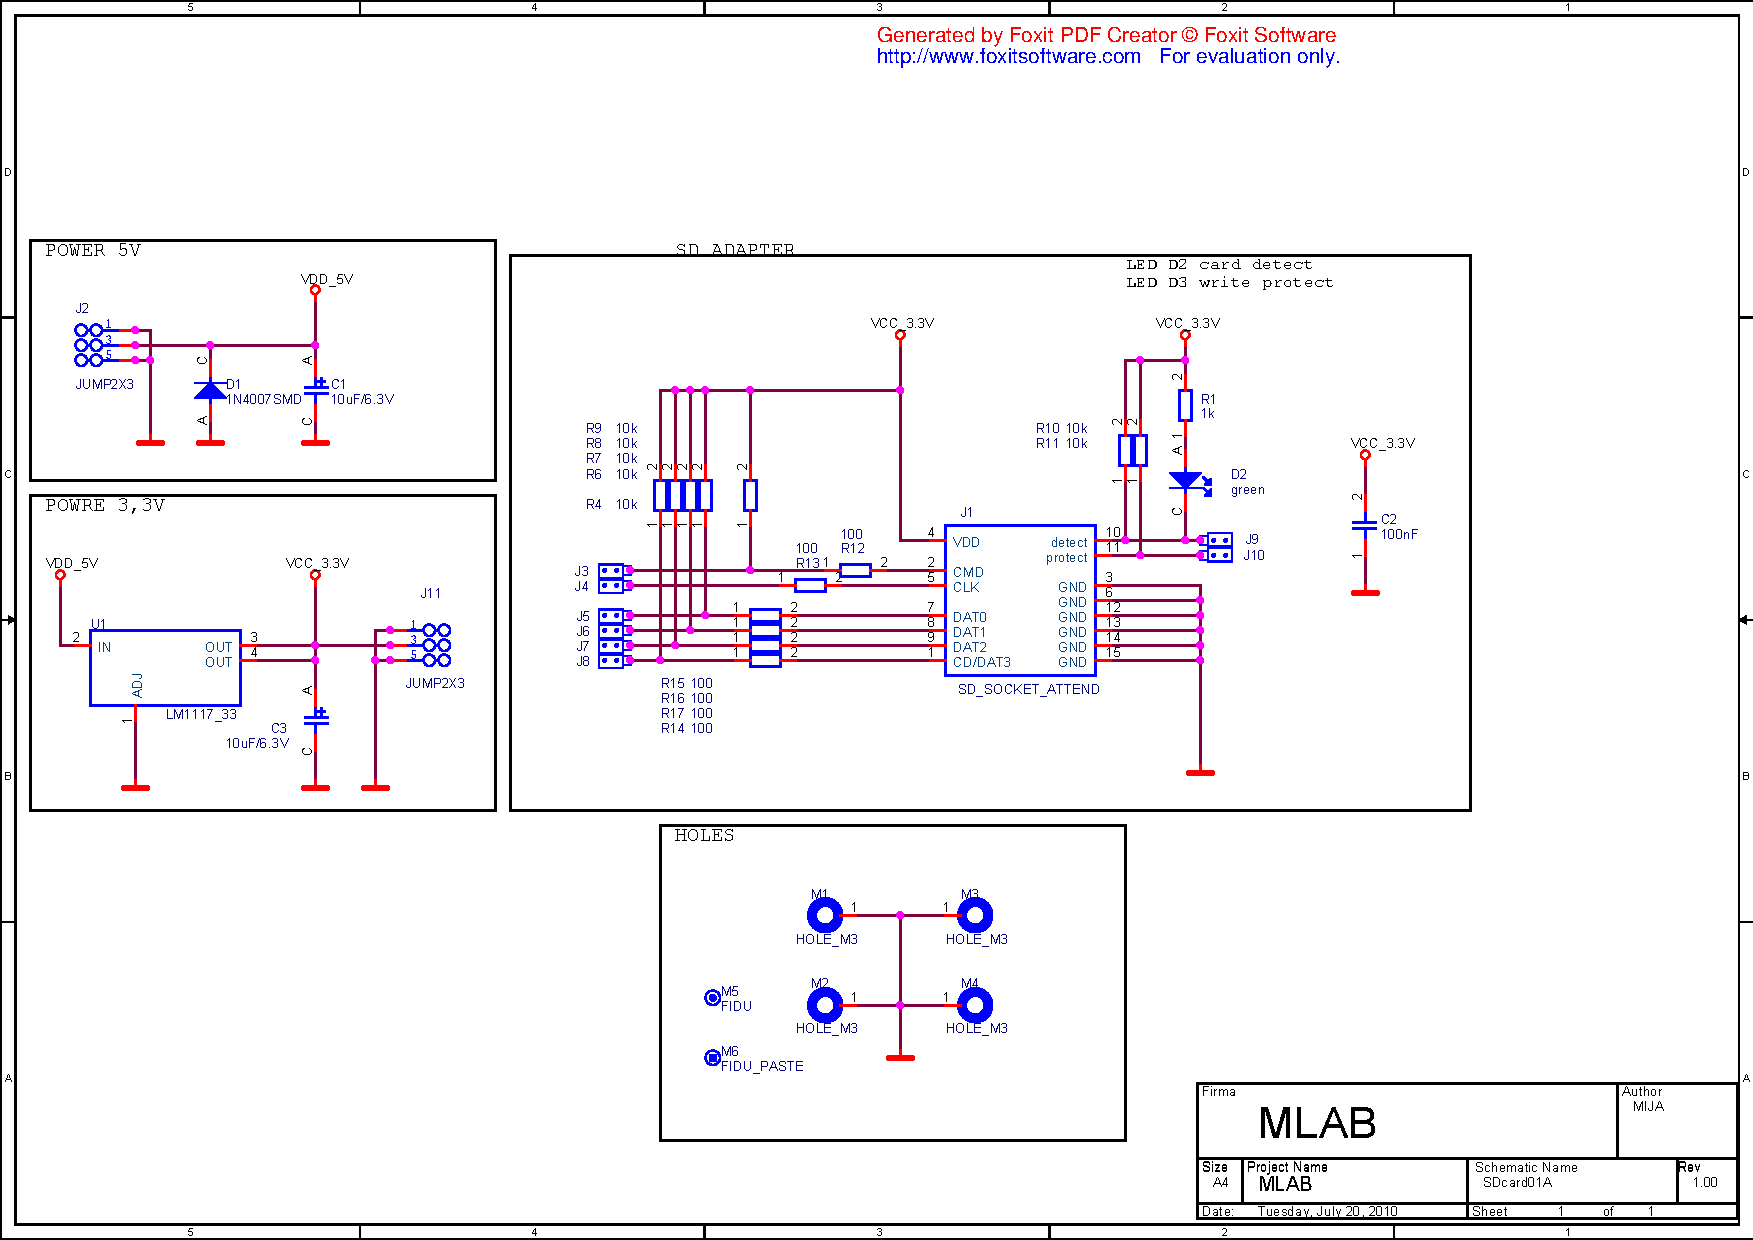
\includepdf[pages={1},landscape=true]{../../SCH/sdcard.pdf}

V zapojení modulu je obsažen lineární stabilizátor určený pro vytvoření napájecího napětí pro SD kartu. Zapojení modulu obsahuje indikační led upozorňující na správné zasunutí SDkarty do slotu. 

\subsection{Mechanická konstrukce}

Modul klasicky předpokládá uchycení na čtyřech šroubech, z důvodu lepšího EMC odstínění je vhodné zabezpečit aby všechny šrouby byly vodivě spojeny s podložkou.  Předpokládá se, že SDkarta bude při použití blíže k základní kovové desce MLAB. 

\section{Výroba a testování}

Plošný spoj je navržen jak pro ruční pájení, tak i pro osazování pomocí pasty.  Modul se testuje optickou kontrolou spojů a následným připojením na laboratorní zdroj s omezením proudu. Lineální stabilizátor by pak na svém výstupu měl dávat zvolené napájecí napětí pro SDkartu. Indikační LED také musí reagovat na přítomnost SDkarty ve slotu. 
Dále je modul testován připojením mikroprocesoru a zápisem na SDkartu.

\subsubsection{Osazení}

Modul je možné osadit i ručně. Rozložení součástek je na Obr. \ref{fig:osazovaci_plan}. Po osazení a zapájení v refrow peci je možné modul umýt v ultrazvukové myčce.  Při použití reflow technologie se předpokládá ruční osazení indikačních LED.

\newpage

\begin{figure} [h!tbp]
  \centering
  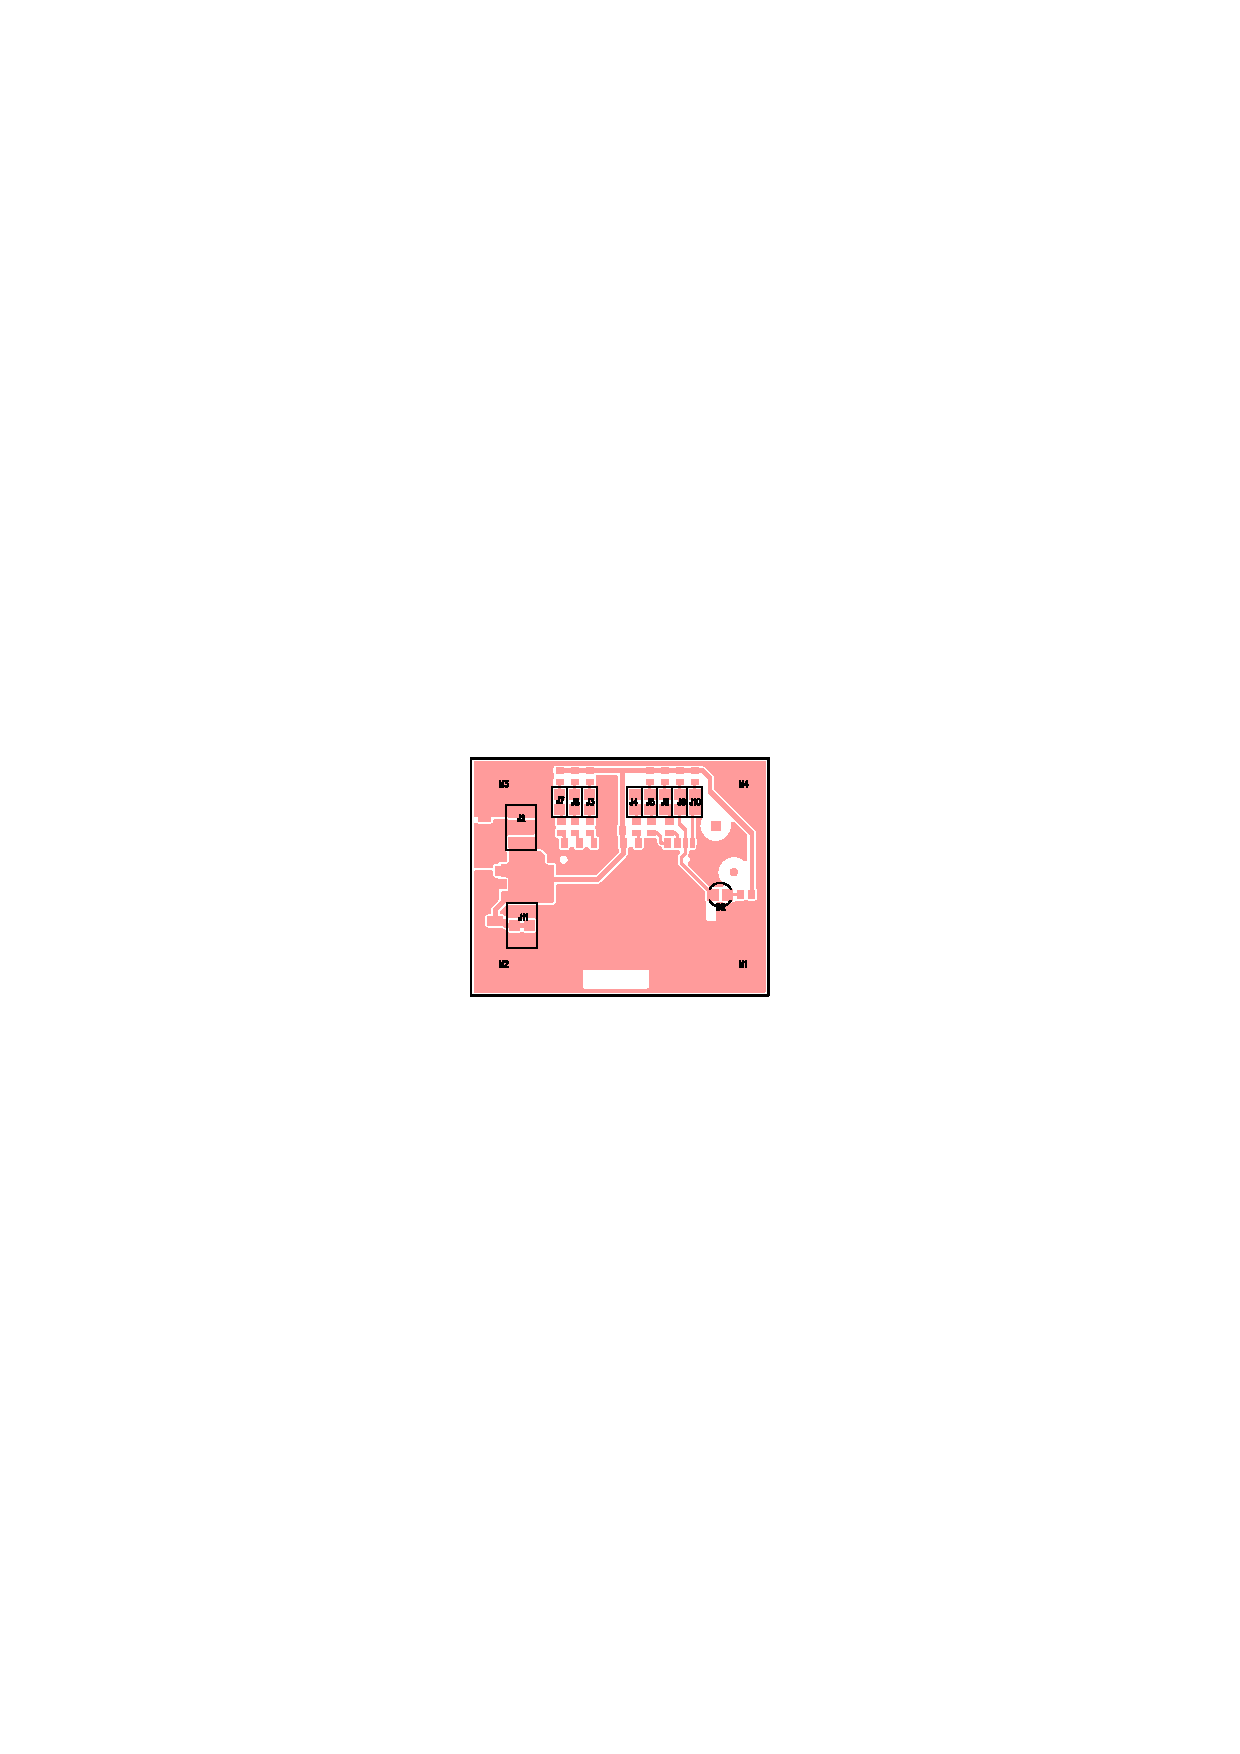
\includegraphics[trim = 7.5cm 12.5cm 7.5cm 12.5cm, clip, width=12cm]{../../CAM_DOC/O1.pdf}
  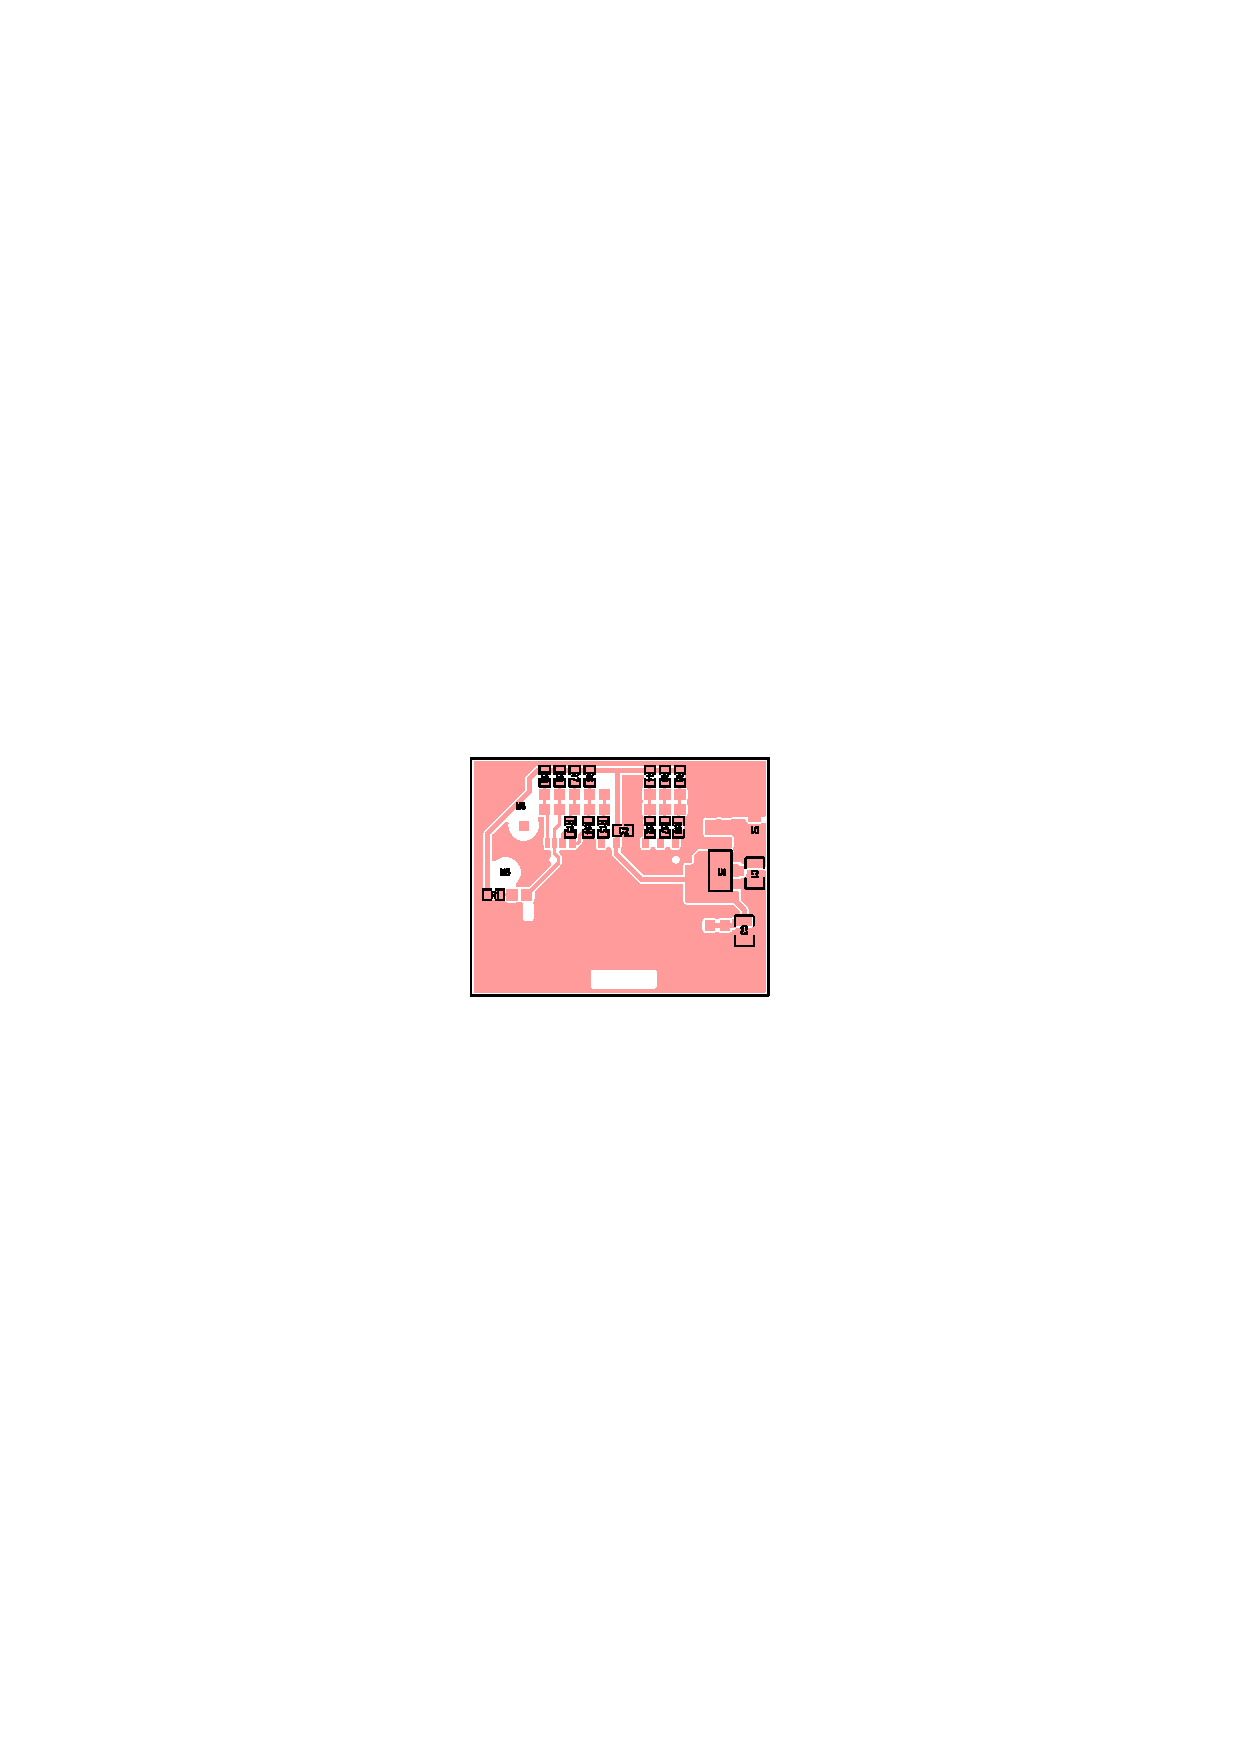
\includegraphics[trim = 7.5cm 12.7cm 7.5cm 12.7cm, clip, width=12cm]{../../CAM_DOC/O2.pdf}
  \caption{Osazovací plán horní a spodní strany plošného spoje}
  \label{fig:osazovaci_plan}
\end{figure}

\begin{savenotes}
\begin{table}[h!]
\begin{center}
\begin{tabular}{ |c|c|c|c| }
\hline 
Počet & Označení & Typ  & Pouzdro  \\ 
\hline 
2	&	C1,C3	&	10uF/6.3V	&	ELYT-B	\\
1	&	C2	&	100nF	&	0805	\\
1	&	D1	&	M4	&	SMA	\\
1	&	D2	&	LED3mm\_green	&		\\
1	&	J1	&	SD\_SOCKET\_ATTEND	&		\\
3	&	J2,J11,(J3,J7,J8)	&	JUMP2X3	&		\\
1	&	(J4,J5,J6,J9,J10)	&	JUMP2X5	&		\\
1	&	R1	&	1k	&	0805	\\
7	&	R4,R6,R7,R8,R9,R10,R11	&	10k	&	0805	\\
6	&	R12,R13,R14,R15,R16,R17	&	100	&	0805	\\
1	&	U1	&	LM1117\_33	&	SOT	\\
4	&	M3 	&	Screw	&		\\
8	&	M3 	&	Nut	&		\\
\hline 
\end{tabular}
\end{center}
\caption{Seznam součástek potřebných pro sestavení modulu.}
\label{seznam_soucastek}
\end{table}
\end{savenotes}

\newpage

\section{Programové vybavení}
K použití modulu lze nejsnáze využít Arduino nebo Wiring knihovny. 

\begin{thebibliography}{99}

\end{thebibliography}
\end{document}